
\documentclass[openany,11pt]{homework}

\coursename{ELEN 4903 Machine Learning (Spring 2018)} % DON'T CHANGE THIS

\studname{Pratyus Pati}    % YOUR NAME GOES HERE
\studmail{pp2636@columbia.edu}% YOUR UNI GOES HERE
\hwNo{5}                   % THE HOMEWORK NUMBER GOES HERE

% Uncomment the next line if you want to use \includegraphics.
\usepackage{graphicx}

\begin{document}
\maketitle

\section*{Problem 1(a)}

\begin{center}
	\centering
	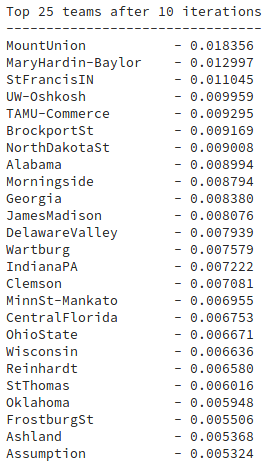
\includegraphics[width = 0.70\textwidth]{1b-10.png}
	\\
	\textbf{Top 25 Teams after $10$ iterations}
\end{center}

\begin{center}
	\centering
	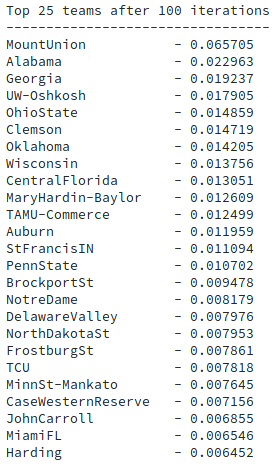
\includegraphics[width = 0.70\textwidth]{1b-100.png}
	\\
	\textbf{Top 25 Teams after $100$ iterations}
\end{center}

\begin{center}
	\centering
	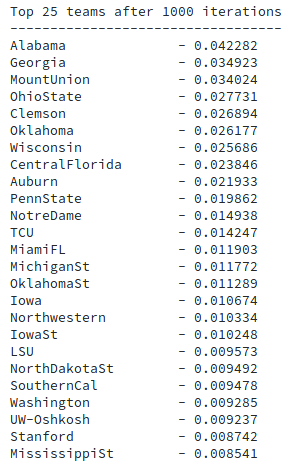
\includegraphics[width = 0.70\textwidth]{1b-1000.png}
	\\
	\textbf{Top 25 Teams after $1000$ iterations}
\end{center}

\begin{center}
	\centering
	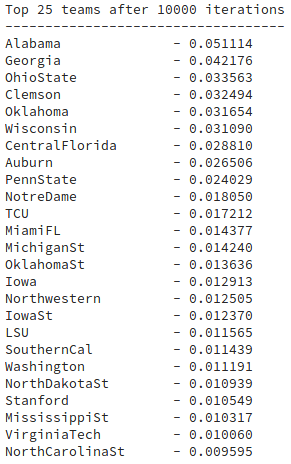
\includegraphics[width = 0.70\textwidth]{1b-10000.png}
	\\
	\textbf{Top 25 Teams after $10000$ iterations}
\end{center}


\section*{Problem 1(b)}
\begin{center}
	\centering
	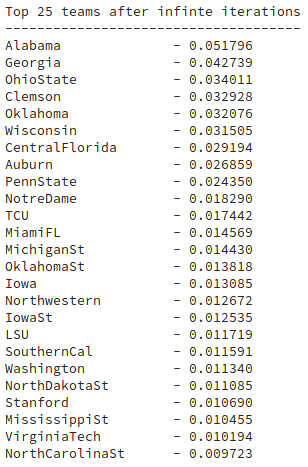
\includegraphics[width = 0.70\textwidth]{1b-inf.png}
	\\
	\textbf{Top 25 Teams based on the stationary distribution}
\end{center}

\begin{center}
	\centering
	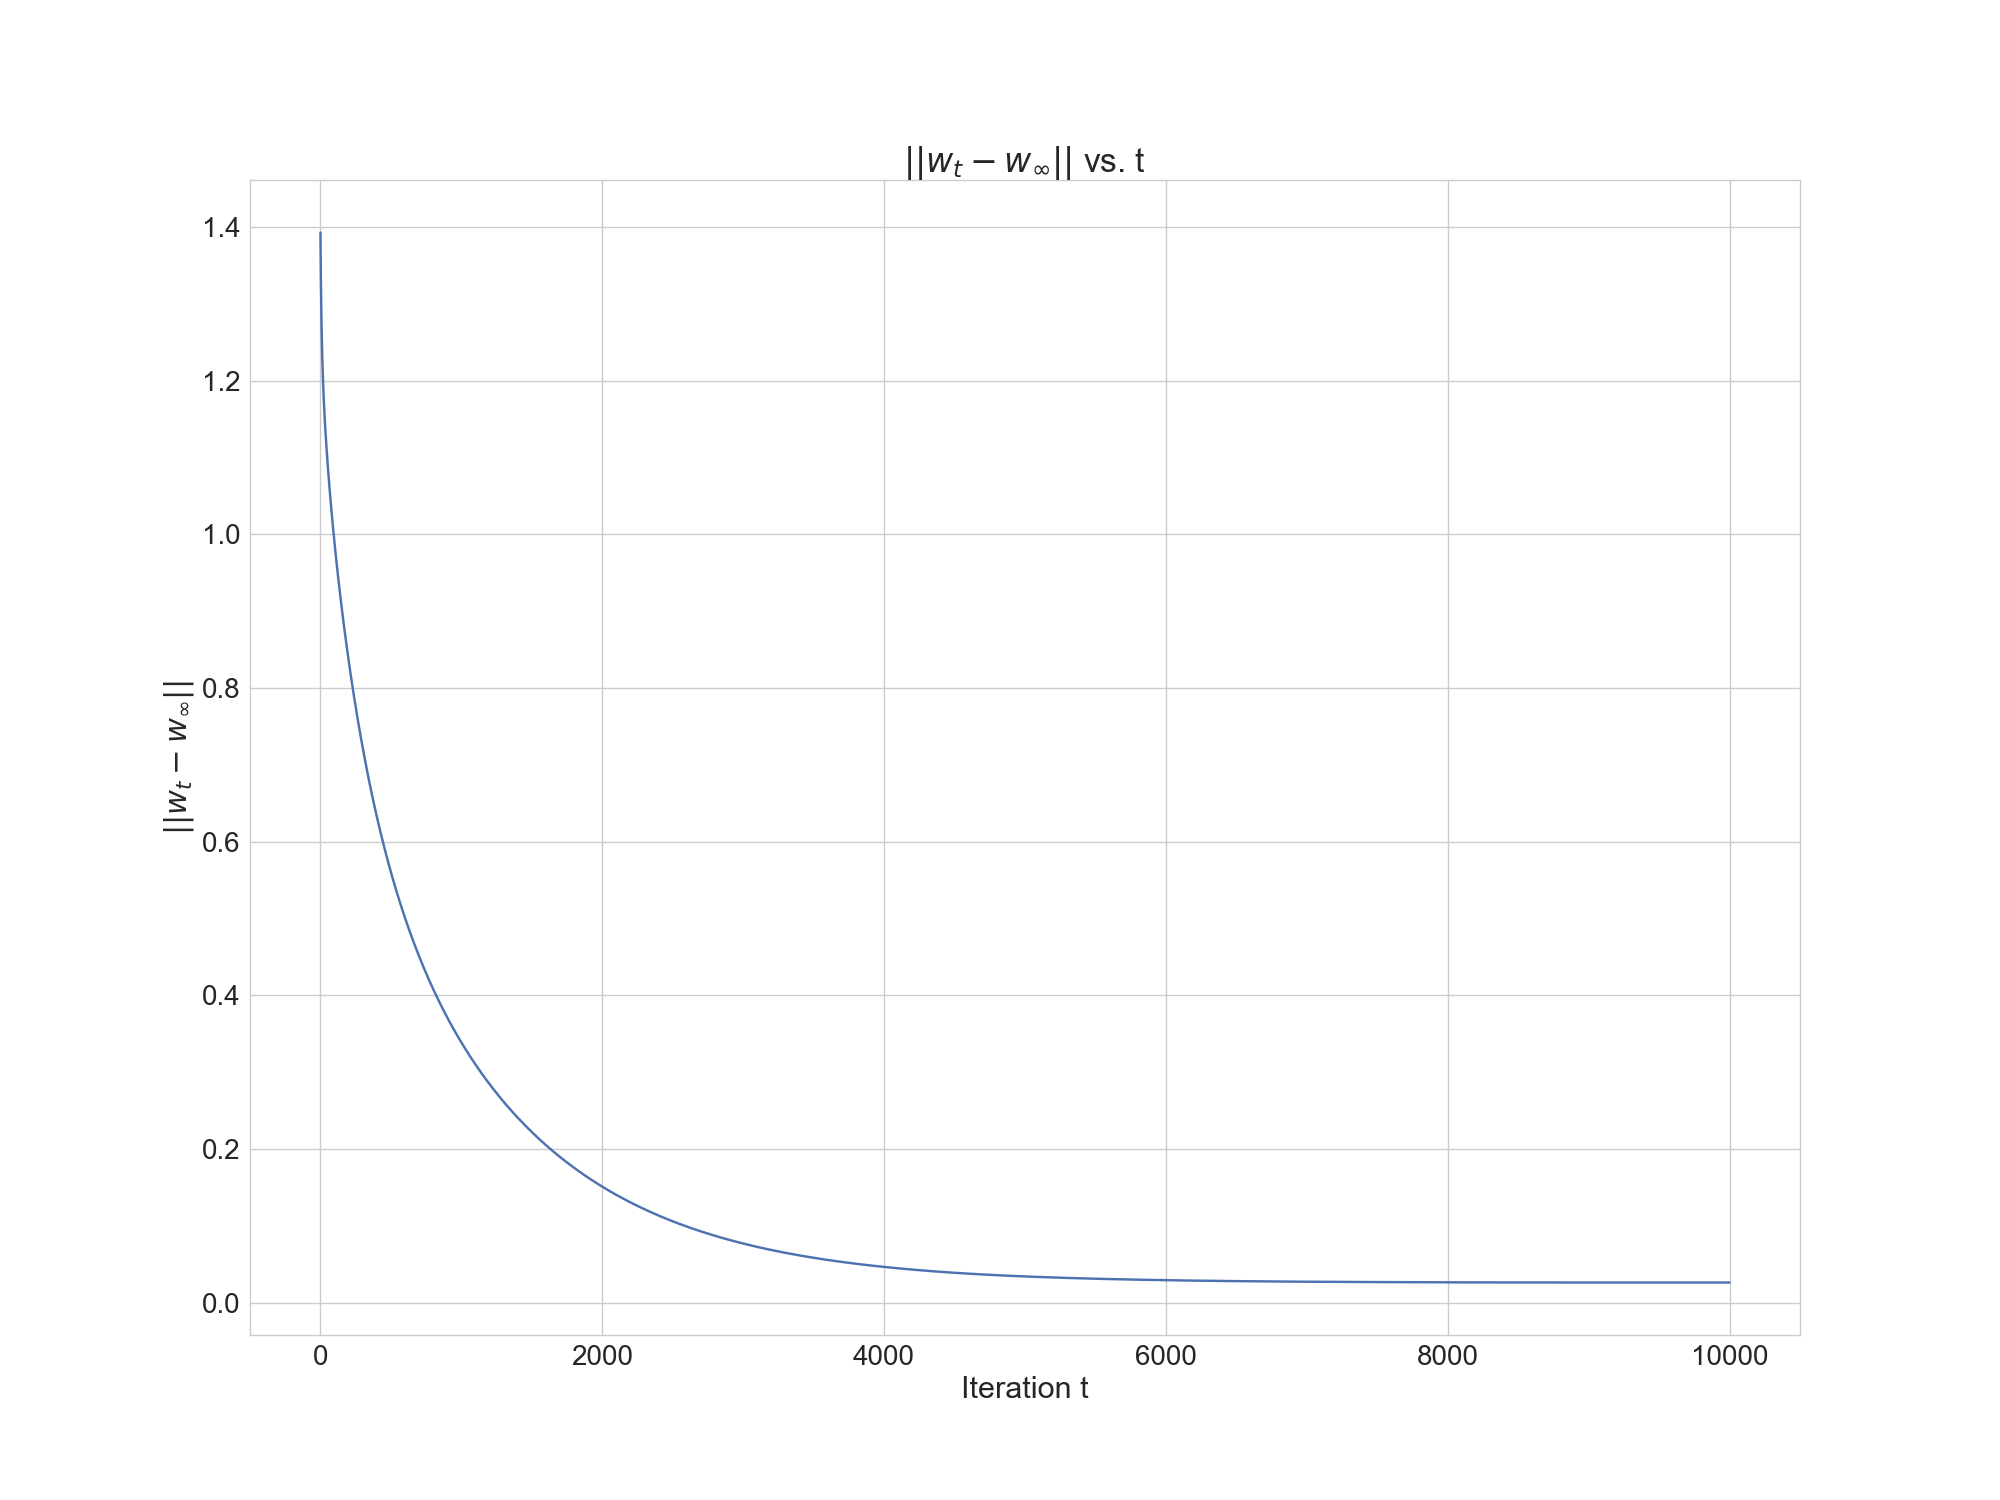
\includegraphics[width = \textwidth]{1a.png}
	\textbf{$\|\|w_t - w_{\infty}\|\|$ vs. Iterations t}
\end{center}


\section*{Problem 2(a)}

\begin{center}
	\centering
	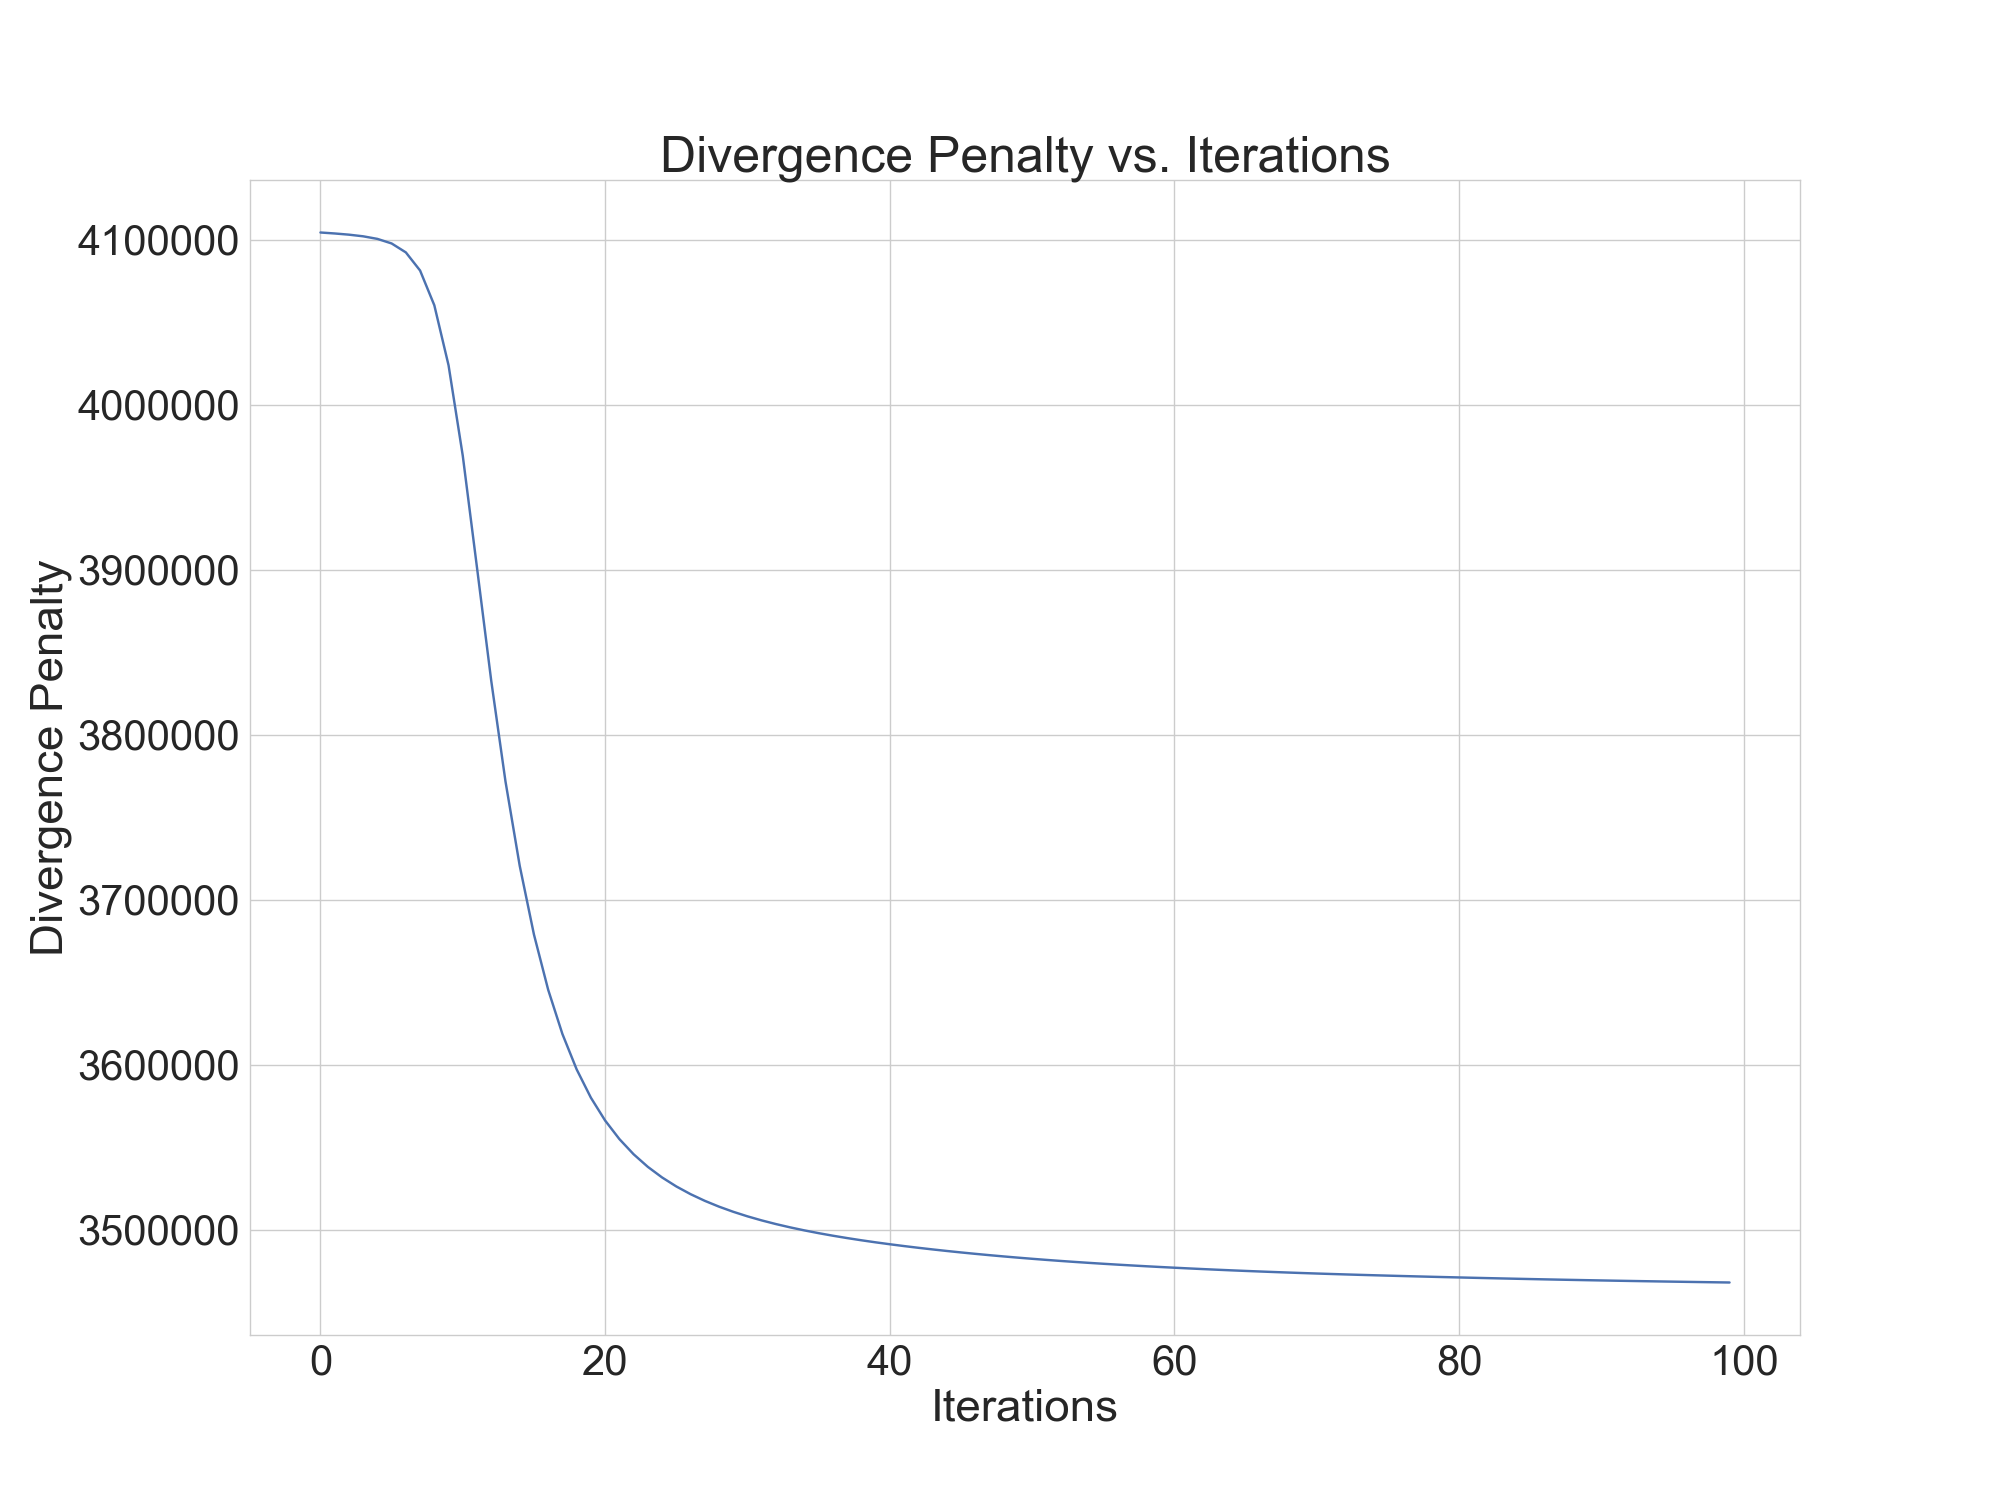
\includegraphics[width = \textwidth]{2a.png}
	\textbf{Divergence Penalty vs Iterations}
\end{center}

\newpage

\section*{Problem 2(b)}

\begin{center}
	\centering
	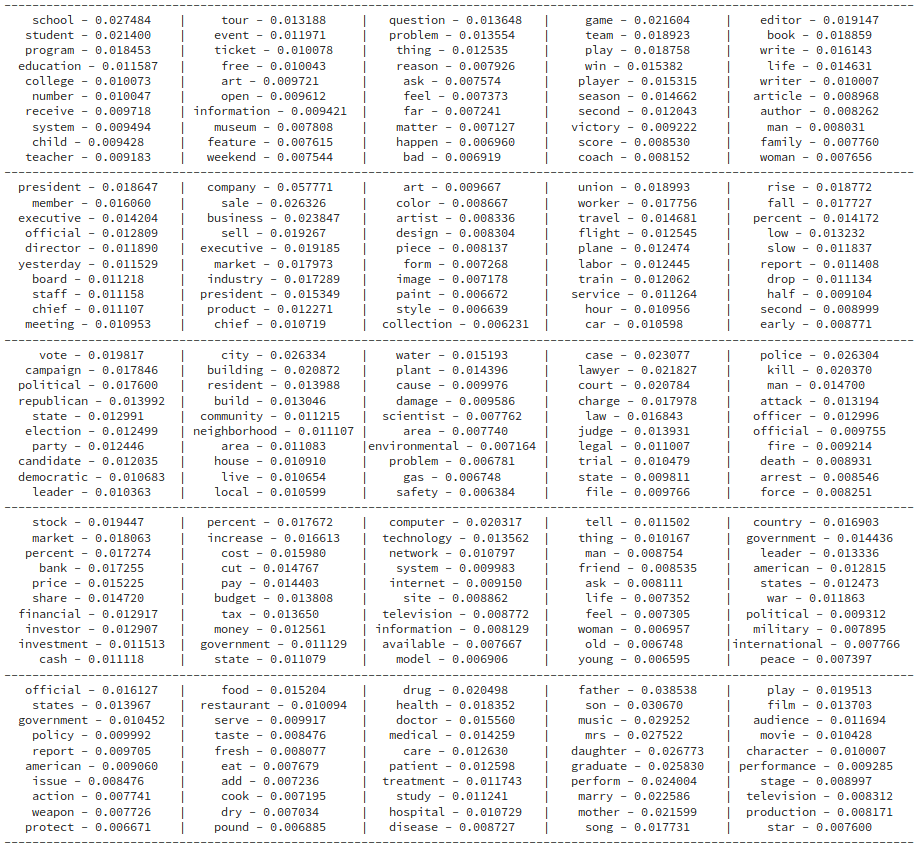
\includegraphics[width = \textwidth]{topics.png}
	\\
	\textbf{Top 10 Words (with scores) per Topic}
\end{center}

\end{document}
